\scanpage{87}
3. \uline{Points fixes de} $\sigma_0,\sigma_1$, \uline{centre} de \uline{la réal. géom.}

\[ \left\{\begin{aligned}\sigma_0(x,y)&=(1-x+\alpha y,y)\\
\sigma_1(x,y)&=(y,x)\\
u(x,y)&=\sigma_0\sigma_1(x,y)=(1-y+\alpha x,x)\end{aligned}\right. \tag*{(26)} \]

\figure{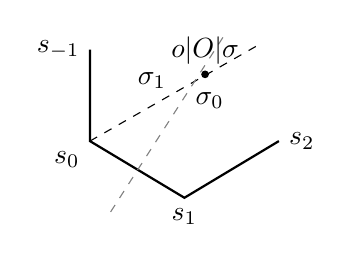
\begin{tikzpicture}[x=.75cm,y=.75cm]
\draw[thick] (0,1.55) node[left] {$s_{-1}$} -- (0,0) node[below left] {$s_0$} -- (1.6,-.96) node[below] {$s_1$} -- (3.2,0) node[right] {$s_2$};
\draw[dashed] (0,0) -- (2.84,1.62);
\draw[thin,gray,dashed] (.35,-1.2) -- (2.30,1.83);
\fill (1.95,1.13) circle (1.4pt) node[above] {$\unsure{o|O|\sigma}$};
\node at (1.05,1.02) {$\sigma_1$}; \node at (2.03,.69) {$\sigma_0$};
\end{tikzpicture}}

Points fixes de $\sigma_0$ :
\[ H_0:\quad 2x-\alpha y-1=0 \tag*{(27)} \]
c'est une droite,
sauf pour $p=2,\alpha=2$
(cas du carré en car. $2$)
où on trouve $H_0=\varnothing$. Mais
\inserted{passant} en coordonnées hom, on
trouve encore une droite
$z=0$ : la droite à l'infini
(Dans ce cas, $\sigma_0$ est la translation par $\deleted{\unsure{e}} e_1$)

Points fixes de $\sigma_1$
\[ H_1:\quad x-y=0 \tag*{(28)} \]
c'est une droite

\uline{NB} Un automorphisme affine \inserted{d'un plan affine} \unsure{dont|que} l'ens des
points fixes est une droite est appelé une
\uline{réflexion affine}. On voit donc que le
cas ``propre'' de la proposition précédente est
caractérisé aussi par la condition

(iv''') $\sigma_0$ est une réflexion affine, ou \deleted{\unsure{à|a}} une
translation \deleted{(dans le} \inserted{(ce dernier cas \deleted{\unsure{seulmt}}} dans le seul cas
$p=2,\alpha=0$ i.e. carré en car. $2$, et alors $\sigma_0$ est
encore une réflexion projective\ldots)
% archive sheet number: 86
